% !TEX root = ../main.tex

\chapter{Related Work}
\label{chapter:RelWork}
There are three aspects relevant to this thesis:
\begin{itemize}
    \item Imitation Learning
    \item Fine Tuning from Sparse Rewards
    \item Learning in POMDPs with a Single Observation
\end{itemize}
. While to the knowledge of the author, there is no approach specifically tailored for all of these aspects, in this chapter we will cover approaches that involve parts 
of the mentioned aspects and can be used with some limitations in our problem setting.

\section{Single Observation Imitation Learning in POMDPs}
The paper "Language-Conditioned Imitation Learning for Robot Manipulation Tasks" \cite{Language-Conditioned Imitation} proposes a method for robot manipulation tasks that takes 
into account natural language instructions. The proposed method involves using a neural network to map natural language instructions to 
corresponding robot actions. The authors also introduce a novel dataset of language-conditioned robot manipulation tasks, which they use to evaluate 
their method. The experimental results demonstrate the effectiveness of their approach in inferring and executing trajectories for robot manipulation 
tasks when language instructions are given.\\

A policy $\pi(v,I)$ is learned to imitate expert behavior in a set of demonstrations $D = \{d_0,...,d_m\}$, each containing a trajectory 
$R \in R^{T \times N}$ over $T$ time steps and with $N$ control variables, an rgb image $I \in \mathcal{R}^{569 \times 320 \times 3}$ of the agent's surroundings, 
and a task description $v \in \mathcal{R}^{15 \times 50}$ from natural language using GloVe \cite{GloVe} embeddings. The proposed method takes the image $I$ and task description $v$ 
to create a task embedding $e$ using GloVe embeddings and a pretrained image recognition model in the semantic model, 
which is subsequently used in the control model to generate robot actions at each time in a closed-loop 
fashion. A schematic overview can be seen in figure \ref{language_imitation}.

Crucially, there is only one observation per trajectory, so we have a POMDP, where we only know the state of the system at time point $t=0$. In this paper, the 
algorithm uses a GRU to ceep track of the former history of the POMDP, similar to the approach described in \ref{POMDP_RNN}. In addition to the hidden state, 
the task embedding $e$ is used in every timestep, as we know, that the task does not change. \\

\begin{figure}[htbp]
    \centering
    \includegraphics[width=\textwidth]{images/Language_Conditioned/System.pdf}
    \caption{Overview of the general system architecture. (Left) Details of the controller model, which
    synthesizes robot control signals . (Right) details of the semantic model, which extracts critical
    information about the task from both perceptual input and language commands. Dark-blue boxes
    indicate pre-trained components of the model \cite{Language-Conditioned Imitation}.}
    \label{language_imitation}
\end{figure}

The learned behaviour consists of picking up objects and pouring their content into other objects. First, a sentense in natural language describes the object, which 
the agent should pick up. For example "Pick up the red cup". This command in combination with the rgb image of the scene is used to generate the trajectory to 
pick up the cup. Then an object is described, into which the robot should pour the content. For example "Pour some of it into the blue bowl". An overview over 
all possible objects and the described example can be found in figure \ref{lang_imi_expl}. The dataset consists of 45 000 tasks, where 4000 tasks are used for 
evaluation and 1000 tasks are used for testing. The authors find that their model can perform $98 \%$ of pick tasks, $85 \%$ of pour tasks and $84 \%$ combined 
tasks, which greatly outperforms a baseline using an end to end RNN model with $58\%$ success rate for picking and $0 \%$ success rate for pouring.

\begin{figure}[htbp]
    \centering
    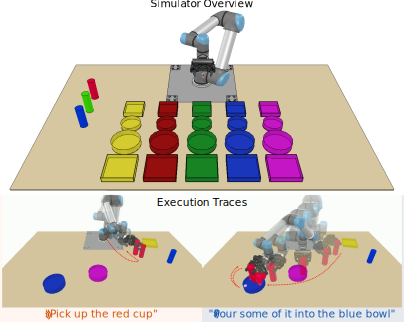
\includegraphics[width=\textwidth]{images/Language_Conditioned/simulator.pdf}
    \caption{Overview of a task. (top) - All possible objects and colors. (left) Example trajectory to "pick up the red cup" following the natural language description. 
    (right) Example trajectory to "pour some of it into the blue bowl". Figure taken from \cite{Language-Conditioned Imitation}.}
    \label{lang_imi_expl}
\end{figure}



\section{Fine Tuning}
\subsection{Sparse Rewards in MDPs}
\subsection{GAIL in POMDPs}